\documentclass{article}
\iffalse
This file is protected by Copyright. Please refer to the COPYRIGHT file
distributed with this source distribution.

This file is part of OpenCPI <http://www.opencpi.org>

OpenCPI is free software: you can redistribute it and/or modify it under the
terms of the GNU Lesser General Public License as published by the Free Software
Foundation, either version 3 of the License, or (at your option) any later
version.

OpenCPI is distributed in the hope that it will be useful, but WITHOUT ANY
WARRANTY; without even the implied warranty of MERCHANTABILITY or FITNESS FOR A
PARTICULAR PURPOSE. See the GNU Lesser General Public License for more details.

You should have received a copy of the GNU Lesser General Public License along
with this program. If not, see <http://www.gnu.org/licenses/>.
\fi

\author{} % Force author to be blank
%----------------------------------------------------------------------------------------
% Paper size, orientation and margins
%----------------------------------------------------------------------------------------
\usepackage{geometry}
\geometry{
	letterpaper,			% paper type
	portrait,				% text direction
	left=.75in,				% left margin
	top=.75in,				% top margin
	right=.75in,			% right margin
	bottom=.75in			% bottom margin
 }
%----------------------------------------------------------------------------------------
% Header/Footer
%----------------------------------------------------------------------------------------
\usepackage{fancyhdr} \pagestyle{fancy} % required for fancy headers
\renewcommand{\headrulewidth}{0.5pt}
\renewcommand{\footrulewidth}{0.5pt}
\rhead{\small{ANGRYVIPER Team}}
%----------------------------------------------------------------------------------------
% Appendix packages
%----------------------------------------------------------------------------------------
\usepackage[toc,page]{appendix}
%----------------------------------------------------------------------------------------
% Defined Commands & Renamed Commands
%----------------------------------------------------------------------------------------
\renewcommand{\contentsname}{Table of Contents}
\renewcommand{\listfigurename}{List of Figures}
\renewcommand{\listtablename}{List of Tables}
\newcommand{\todo}[1]{\textcolor{red}{TODO: #1}\PackageWarning{TODO:}{#1}} % To do notes
\newcommand{\code}[1]{\texttt{#1}} % For inline code snippet or command line
%----------------------------------------------------------------------------------------
% Various pacakges
%----------------------------------------------------------------------------------------
\usepackage{hyperref} % for linking urls and lists
\usepackage{graphicx} % for including pictures by file
\usepackage{listings} % for coding language styles
\usepackage{rotating} % for sideways table
\usepackage{pifont}   % for sideways table
\usepackage{pdflscape} % for landscape view
%----------------------------------------------------------------------------------------
% Table packages
%----------------------------------------------------------------------------------------
\usepackage{longtable} % for long possibly multi-page tables
\usepackage{tabularx} % c=center,l=left,r=right,X=fill
\usepackage{float}
\floatstyle{plaintop}
\usepackage[tableposition=top]{caption}
\newcolumntype{P}[1]{>{\centering\arraybackslash}p{#1}}
\newcolumntype{M}[1]{>{\centering\arraybackslash}m{#1}}
%----------------------------------------------------------------------------------------
% Block Diagram / FSM Drawings
%----------------------------------------------------------------------------------------
\usepackage{tikz}
\usetikzlibrary{shapes,arrows,fit,positioning}
\usetikzlibrary{automata} % used for the fsm
%----------------------------------------------------------------------------------------
% Colors Used
%----------------------------------------------------------------------------------------
\usepackage{colortbl}
\definecolor{blue}{rgb}{.7,.8,.9}
\definecolor{ceruleanblue}{rgb}{0.16, 0.32, 0.75}
\definecolor{drkgreen}{rgb}{0,0.6,0}
\definecolor{deepmagenta}{rgb}{0.8, 0.0, 0.8}
\definecolor{cyan}{rgb}{0.0,0.6,0.6}
\definecolor{maroon}{rgb}{0.5,0,0}
%----------------------------------------------------------------------------------------
% Update the docTitle and docVersion per document
%----------------------------------------------------------------------------------------
\def\docTitle{Component Data Sheet}
\def\docVersion{1.5}
%----------------------------------------------------------------------------------------

\usepackage{listings}

\date{Version \docVersion} % Force date to be blank and override date with version
\title{\docTitle}
\lhead{\small{\docTitle}}

\def\comp{real\_digitizer}
\edef\ecomp{real_digitizer}
\def\Comp{Real Digitizer}
\graphicspath{ {figures/} }

\begin{document}

\section*{Summary - \Comp}
\begin{tabular}{|c|M{13.5cm}|}
	\hline
	\rowcolor{blue}
	                  &                                          \\
	\hline
	Name              & \comp                                    \\
	\hline
	Worker Type       & Application                              \\
	\hline
	Version           & v\docVersion \\
	\hline
	Release Date      & April 2019 \\
	\hline
	Component Library & ocpi.assets.dsp\_comps                    \\
	\hline
	Workers           & \comp.rcc                                \\
	\hline
	Tested Platforms  & centos7, xilinx13\_3, xilinx13\_4 \\
	\hline
\end{tabular}
\begin{center}
  \textit{\textbf{Revision History}}
\end{center}
\begin{tabular}{|p{2cm}|p{12cm}|p{2.11cm}|}
  \hline
  \rowcolor{blue}
  \textbf{Revision} & \textbf{Description of Change} & \textbf{Date} \\
  \hline
  v1.0 & Initial release. & 2/2016 \\
  % If you look through the git history, this file appears to have undergone a
  % 'git mv' such that it was associated with an entirely different component,
  % and then another 'git mv' to revert back. These moves occurred before 1.1 and
  % after 1.3 releases, so it appears that this datasheet for real digitizer
  % didn't even exist for releases 1.1, 1.2, and 1.3.
  \hline
  v1.4 & Updated formatting, block diagram, and performance and resource utilization. Updated source dependencies to reflect new assets project directory name. & 9/2018 \\
  \hline
  v1.5 & Added \verb+enable_printing+ and \verb+sync_criteria_met+ properties to \comp{}.rcc. Also added functional diagram and xilinx13\_4 as a tested platform. & 4/2019 \\
  \hline
\end{tabular}

\section*{Worker Implementation Details}
\subsection*{\comp.rcc}
This worker performs symbol decisions by decoding signed real Q0.15 symbols into bits. Each positive symbol is decoded to a 1 and each negative symbol is decoded into a 0.
Once the sync criteria is met, the decoded bits are packed into 16-bit words which are subsequently sent to the output port.
The sync criteria is met when a) the \verb+need_sync+ property has a value of false, or b) the first 0xFACE sequence occurs in the decoded bits. When the first 0xFACE sequence occurs in the decoded bits and the \verb+enable_printing+ is true, the following is printed to stdout:
\lstset{language=bash, backgroundcolor=\color{lightgray}, columns=flexible,
        breaklines=true, prebreak=\textbackslash, basicstyle=\ttfamily,
        showstringspaces=false,upquote=true, aboveskip=\baselineskip,
        belowskip=\baselineskip}
\begin{lstlisting}
sync pattern 0xFACE found
\end{lstlisting}

\section*{Block Diagrams}
\subsection*{Top level}
\begin{center}
	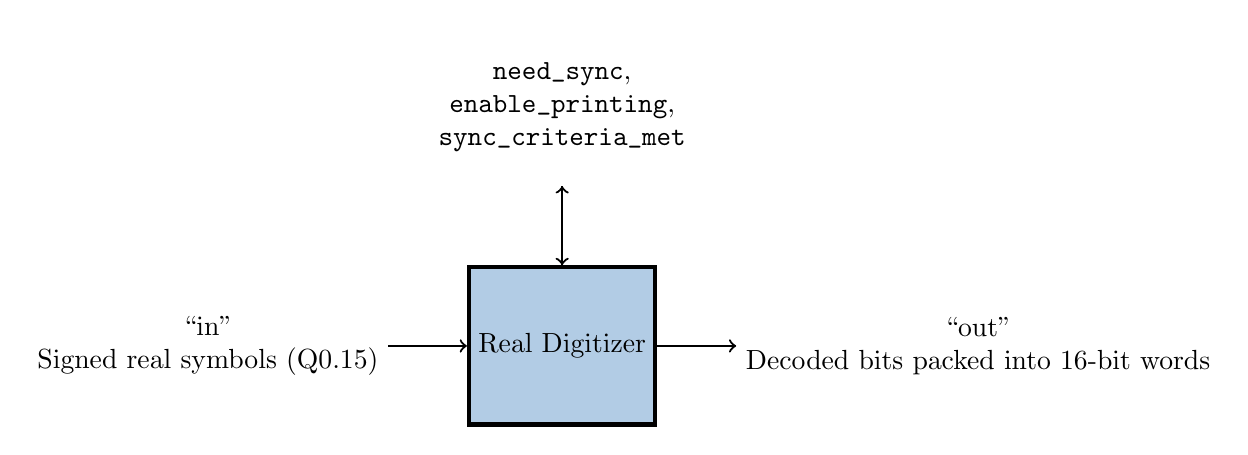
\begin{tikzpicture}[% List of styles applied to all, to override specify on a case-by-case
			every node/.style={
				align=center,  		% use this so that the "\\" for line break works
				minimum size=2cm	% creates space above and below text in rectangle
			},
			every edge/.style={draw,thick}
		]
		\node[rectangle,ultra thick,draw=black,fill=blue](R2){\Comp};
		\node[rectangle,draw=white,fill=white](R3)[left= of R2]{``in'' \\ Signed real symbols (Q0.15)};
		\node[rectangle,draw=white,fill=white](R4)[right= of R2]{``out'' \\ Decoded bits packed into 16-bit words};
		\node[rectangle,draw=white,fill=white](R5)[above= of R2]{\verb+need_sync+, \\ \verb+enable_printing+, \\ \verb+sync_criteria_met+};
		\path[->]
		(R3)edge []	node [] {} (R2)
		(R2)edge []	node [] {} (R4)
		(R2)edge []	node [] {} (R5)
		(R5)edge []	node [] {} (R2)
		;
	\end{tikzpicture}
  \captionof{figure}{\comp{}.rcc Worker Diagram}
\end{center}

\begin{center}
  \begin{figure}[h]
    \centering\captionsetup{type=figure}\includegraphics[scale=0.14]{Real_Digitizer_Diagram}
    \captionof{figure}{\comp{}.rcc Functional Diagram}
    \label{fig:blockdiagram}
  \end{figure}
\end{center}



\section*{Source Dependencies}
\subsection*{\comp.rcc}
\begin{itemize}
	\item projects/assets/components/dsp\_comps/\comp.rcc/\comp.c
\end{itemize}

\begin{landscape}
	\section*{Component Spec Properties}
	\begin{scriptsize}
		\begin{tabular}{|p{3cm}|p{1.5cm}|c|c|c|c|c|p{7cm}|}
			\hline
			\rowcolor{blue}
			Name             & Type & SequenceLength & ArrayDimensions & Accessibility    & Valid Range & Default & Usage                                                                                                                                                                                \\
			\hline
			\verb+need_sync+ & Bool & -              & -               & Readable,Initial & Standard    & True    & When set to true the worker will look for the initialization sequence 0xFACE in the data stream before sending data to the next worker. When set to false, all data is passed along. \\
			\hline
		\end{tabular}
	\end{scriptsize}

	\section*{Worker Properties}
	\subsection*{\comp.rcc}
	Control Operations: Start \\ \\
	\begin{scriptsize}
		\begin{tabular}{|p{3cm}|p{1.5cm}|c|c|c|c|c|p{7cm}|}
			\hline
			\rowcolor{blue}
			Name             & Type & SequenceLength & ArrayDimensions & Accessibility    & Valid Range & Default & Usage                                                                                                                                                                                \\
			\hline
			\verb+enable_printing+ & Bool & -              & -               & Writable & Standard    & True    & Enable stdout/stderr printing. \\
			\hline
			\verb+sync_criteria_met+ & Bool & -              & -               & Volatile & Standard    & -       & Indicates either 0xFACE found or \verb+need_sync+ is false. \\
			\hline
		\end{tabular}
	\end{scriptsize}

	\section*{Component Ports}
	\begin{scriptsize}
		\begin{tabular}{|M{2cm}|M{1.5cm}|M{4cm}|c|c|M{9cm}|}
			\hline
			\rowcolor{blue}
			Name & Producer & Protocol          & Optional & Advanced & Usage               \\
			\hline
			in   & false    & rstream\_protocol & false    & -        & Signed real symbols (Q0.15) \\
			\hline
			out  & true     & rstream\_protocol & false    & -        & Decoded bits packed in 16-bit words \\
			\hline
		\end{tabular}
	\end{scriptsize}
\end{landscape}

\section*{Test and Verification}
\normalsize
No unit test currently exists for this worker.
\end{document}
